% https://www.tinkercad.com/things/5tth6OLRHPt-copy-of-kit-logico-modelo/editel?sharecode=SUnxTp9Fps-BiMfSit7VU2lw1o5RQNifgeI15UbR-yM
% https://www.tinkercad.com/things/hCCrtzcJJyE-roteiro3-parte-22/editel?sharecode=PtsZp45ElX69eXlrZ6RUbpy1vHVZd_---8yJ6dxY2TU
% https://www.tinkercad.com/things/69kCawlKX2i-roteiro3-parte-23/editel?sharecode=3Xug60JRRaJmdqFbfj94RdsFyIY3DcZ6AZmUIQGJKSs
% https://drive.google.com/drive/folders/1qmQaSxEHMEMgjFNUYUIII_uWlMOWUh7Z?usp=sharing

%%%%%%%%%%%%%%%%%%%%%%%%%%%%%%%%%%%%%%%%%%%%%%%%%%%%%%%%
% Este é um documento que servirá de modelo para
% os relatórios feitos na disciplina Laboratório de Circuitos Lógicos
% 2020-2
%%%%%%%%%%%%%%%%%%%%%%%%%%%%%%%%%%%%%%%%%%%%%%%%%%%%%%%%%

%%%%%%%%%%%%%%%%%%%%%%%%%%%%%%%%%%%%%%%%%%%%%%%%%%%%%%%%%
% Use os diferentes diretórios para colocar os relatórios de cada experimento, deste modo vc consegue manter um histórico e todo material organizado em apenas um local.
% Lembre-se de mudar o Main Document no Menu!!!

\documentclass[12pt]{article}

\usepackage{sbc-template}
\usepackage[brazil,american]{babel}
\usepackage[utf8]{inputenc}

\usepackage{graphicx}
\usepackage{url}
\usepackage{float}
\usepackage{listings}
\usepackage{color}
\usepackage{todonotes}
\usepackage{algorithmic}
\usepackage{algorithm}
\usepackage{hyperref}
\usepackage{amsmath}
\usepackage{graphicx}
\usepackage{array}

\sloppy


\title{Experimento 3\\
Circuitos Combinacionais: Mapa de Karnaugh}

\author{Matheus Cardoso de Souza, 202033507\\
        Ualiton Ventura da Silva, 202033580\\
        Grupo G42
}

%%%% LEMBRE-SE DE MUDAR O GRUPO NA LINHA ABAIXO!!!!! %%%%%%
\address{Dep. Ciência da Computação -- Universidade de Brasília (UnB)\\
  CIC0231 - Laboratório de Circuitos Lógicos
  \email{matheus-cardoso.mc@aluno.unb.br, 202033580@aluno.unb.br}
}

\begin{document}
\maketitle

\selectlanguage{american}
 \begin{abstract}
   This report corresponds to the Experiment 3 on ``Combinational Circuits: \textbf{Karnaugh Map}''. With this experiment we were able to more broadly applly and understand \textbf{NAND} gate's property of functional completeness, applying only this logic gate to build a Majority Decision Circuitry, as well as a Minority Decision and a Equality Decision Circuitry.
 \end{abstract}
\selectlanguage{brazil}

 \begin{resumo}
  O presente relatório corresponde ao Experimento 3 sobre ``Circuitos Combinacionais: \textbf{Mapa de Karnaugh}''. Com esse experimento pudemos aplicar e entender mais amplamente a propriedade de completude funcional das portas lógicas \textbf{NAND}, aplicando somente elas para criar três circuitos: Decisão de Maioria, Minoria e Igualdade.
 \end{resumo}


\section{Introdução}
\label{sec:Introducao}

% Escreva com suas palavras o que vai ser trabalhado no experimento. Aqui temos um exemplo de como citar a bibliografia consultada \cite{boulic:91} \cite{smith:99}.

Os experimentos realizados neste experimento visam abordar assuntos como a
criação de circuitos combinacionais utilizando minimização lógica através de
mapas de Karnaugh. Além disso, exploraremos a universalidade e completude das
portas \textbf{NAND} para a construção de qualquer circuito lógico desejado.

Cabe observar que, valendo-se do uso de ferramentas de simplificação lógica como
o mapa de Karnaugh (ou o algoritmo de Quine–McCluskey, não abordado nesse
experimento), podemos não somente facilitar a construção de circuitos lócicos,
mas também reduzir gastos com componentes físicos, pois a minimização lógica em
grande maioria dos casos, leva a um uso de menos portas lógicas, facilitando
tando a vida do programador que precisa organizar os circuitos que devem ser
montados, como o poupa da necessidade de arcar com outros circuitos integrados
caso fosse implementar uma função lógica menos otimizada.

\subsection{Objetivos}
\label{sec:Objetivos}
Neste experimento temos como objetivo abordar conceitos referentes ao uso de
mapas de Karnaugh para a simplificação de funções booleanas, a fim de
proporcionar a criação de circuitos combinacionais mais simples e eficientes.

\subsection{Materiais}
\label{sec:Materiais}
Em função da natureza do ensino a distância, os presentes experimentos não foram
realizados usando-se materiais e equipamentos físicos, mas sim emulados por meio
do simulador online \href{https://www.tinkercad.com/}{Tinkercad}, e também do
\href{https://www.digitalelectronicsdeeds.com/deeds.html}{Deeds}.

A seguir estão enumerados os materiais simulados:
\begin{itemize}
    \item Painel Digital
    \item \textit{Protoboard}
    \item Fios
    \item Seletores de estado lógico
    \item LEDs
    \item Resistores
    \item Multímetros
    \item Portas Lógicas \textbf{NAND}
\end{itemize}

\section{Procedimentos}
\label{sec:Procedimentos}

Passaremos a apresentar os experimentos requeridos.

\subsection{Circuito para \textit{``Decisão de Maioria''} utilizando apenas portas \textbf{NAND}}\label{sec:decisao_maioria}

O atual experimento visa implementar um circuito para \textit{Decisão de
Maioria} utilizando somente portas \textbf{NAND}. O circuito deve ter 4 inputs
(\textbf{A}, \textbf{B}, \textbf{C} e \textbf{D}) e ter como output uma saída em
LED (\(Y_{1}\) \( = \) \textbf{L0}).

Como desejamos fazer uma decisão de maioria, precisamos inicialmente planejar
qual circuito lógico produziria o resultado desejado. Assim, precisamos
inicialmente construir a tabela verdade desejada, que será a seguinte:

\begin{table}[H]
    \centering
    \caption{Tabela Verdade para Decisão de Maioria}
    \begin{tabular}{|c|c|c|c|c|}\hline
    \multicolumn{4}{|c|}{Entradas} & \multicolumn{1}{|c|}{Saída} \\\hline
    \textbf{D} & \textbf{C} & \textbf{B} & \textbf{A} & $\textbf{L0}=Y_{1}$ \\\hline
    0 & 0 & 0 & 0 & 0 \\\hline
    0 & 0 & 0 & 1 & 0 \\\hline
    0 & 0 & 1 & 0 & 0 \\\hline
    0 & 0 & 1 & 1 & 0 \\\hline
    0 & 1 & 0 & 0 & 0 \\\hline
    0 & 1 & 0 & 1 & 0 \\\hline
    0 & 1 & 1 & 0 & 0 \\\hline
    0 & 1 & 1 & 1 & 1 \\\hline
    1 & 0 & 0 & 0 & 0 \\\hline
    1 & 0 & 0 & 1 & 0 \\\hline
    1 & 0 & 1 & 0 & 0 \\\hline
    1 & 0 & 1 & 1 & 1 \\\hline
    1 & 1 & 0 & 0 & 0 \\\hline
    1 & 1 & 0 & 1 & 1 \\\hline
    1 & 1 & 1 & 0 & 1 \\\hline
    1 & 1 & 1 & 1 & 1 \\\hline
    \end{tabular}\label{tab:tabela_and}
\end{table}

De posse da tabela verdade, podemos criar uma fórmula booleana que retorne o
output desejado. Criando o mapa de Karnaugh para essa tabela verdade, observamos
o seguinte:

\emph{Obs: Utilizamos a ferramenta referênciada em \cite{karnaugh_generator} para
criar esse e os seguintes mapas de karnaugh.}

\begin{figure}[H]
    \centering
    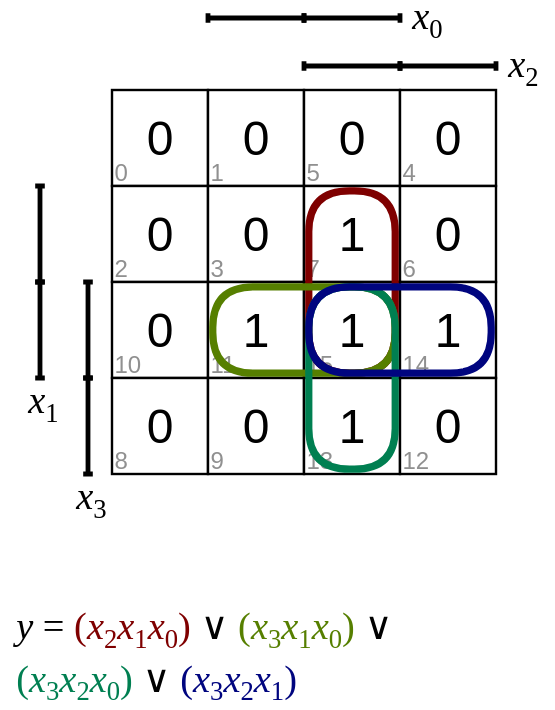
\includegraphics[width=.5\textwidth]{Exp03/2_1_karnaugh_map.png}
    \caption{Mapa de Karnaugh para o \textit{``Circuito de Maioria''}}\label{fig:2_1_karnaugh_map.png}
\end{figure}

Observando o mapa de Karnaugh, vemos que, por \textit{Soma de Produtos}, temos a seguinte equação para \(Y_{1}\):

\begin{equation}
  Y_{1} = (ABC) + (ABD) + (ACD) + (BCD)
\end{equation}

Entretanto, como devemos representar essa fórmula apenas em termos de portas
\textbf{NAND}, precisamos modificar a equação um pouco. Também temos a questão
de que esse circuito seria muito complexo para se implementar usando uma
conversão direta das portas usadas na \textit{``Figura 10''} do roteiro por
portas \textbf{NAND} requeridas no enunciado. Por isso, também realizaremos
alguns passos para minimização da função booleana.

\begin{align}
  Y_{1} &= (ABC) + (ABD) + (ACD) + (BCD)\\
  Y_{1} &= AB \cdot (C + D) + CD \cdot (A + B)\\
  Y_{1} &= AB \cdot (\overline{\overline{C}} + \overline{\overline{D}}) + CD \cdot (\overline{\overline{A}} + \overline{\overline{B}})\\
  Y_{1} &= AB \cdot \overline{ \left( \overline{C} \cdot \overline{D} \right) } + CD \cdot \overline{ \left( \overline{A} \cdot \overline{B} \right) }\\
  Y_{1} &= \overline{ \overline{ \left[ AB \cdot \overline{ \left( \overline{C} \cdot \overline{D} \right) } \right] } } + \overline{ \overline{ \left[ CD \cdot \overline{ \left( \overline{A} \cdot \overline{B} \right) } \right] } } \\
  Y_{1} &= \overline{ \left\{ \overline{ \left[AB \cdot \overline{ \left( \overline{C} \cdot \overline{D} \right) } \right] } \cdot \overline{ \left[ CD \cdot \overline{ \left( \overline{A} \cdot \overline{B} \right) } \right] } \right\} } \label{eq:2.1_NAND}
\end{align}

Possuindo a fórmula final \ref{eq:2.1_NAND} para o resultado \(Y_{1}\) desejado,
podemos criar um diagrama de mapeamento da função booleana para o circuito
lógico final:

\begin{figure}[H]
    \centering
    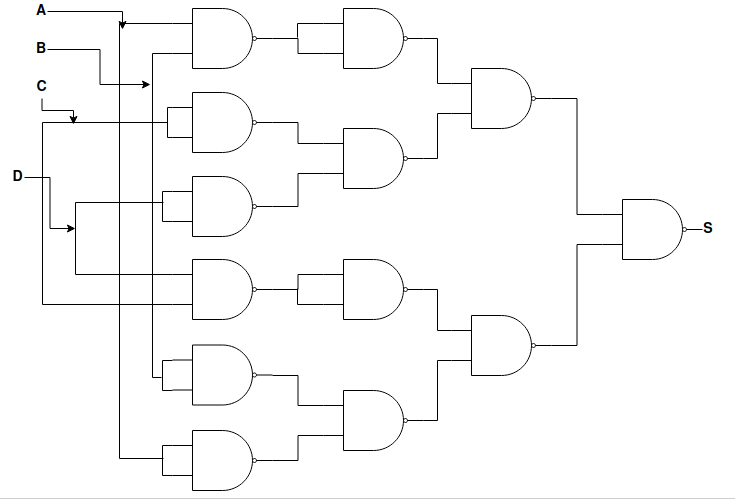
\includegraphics[width=.85\textwidth]{Exp03/2.1.png}
    \caption{Decisão de Maioria apenas com portas \textbf{NAND}}
    \label{fig:decisao_maioria}
\end{figure}

É possível concluir através da tabela, do diagrama, e da fórmula em
\ref{eq:2.1_NAND}, que de fato o circuito lógico final descreve uma decisão de
maioria com \(4\) entradas utilizando apenas usando portas \textbf{NAND}.

Como requisitado, apresentamos a montagem do circuito abaixo:

\begin{figure}[H]
    \centering
    \includegraphics[width=.9\textwidth]{Exp03/2.1_montagem.jpg}
    \caption{Montagem do circuito para \textit{Decisão de Maioria} apenas com portas \textbf{NAND}}
    \label{fig:decisao_maioria_montagem}
\end{figure}

Para conferir o vídeo deste experimento, acesse o seguinte link:
\href{https://youtu.be/TXYnvVoP6OI}{https://youtu.be/TXYnvVoP6OI}.
\\[2em]

\subsection{Circuito para \textit{``Decisão de Minoria''} utilizando apenas portas \textbf{NAND}}\label{sec:decisao_minoria}

O atual experimento visa implementar um circuito para \textit{Decisão de
Minoria} utilizando somente portas \textbf{NAND}. O circuito deve ter 4 inputs
(\textbf{A}, \textbf{B}, \textbf{C} e \textbf{D}) e ter como output uma saída em
LED (\(Y_{2}\) \( = \) \textbf{L1}).

Esse experimento é muito semelhante ao anterior. Dessa forma, seguiremos os
mesmos passos:

Como desejamos fazer uma decisão de minoria, precisamos inicialmente planejar
qual circuito lógico produziria o resultado desejado. Assim, precisamos
inicialmente construir a tabela verdade desejada, que será a seguinte:

\begin{table}[H]
    \centering
    \caption{Tabela Verdade para Decisão de Minoria}
    \begin{tabular}{|c|c|c|c|c|}\hline
    \multicolumn{4}{|c|}{Entradas} & \multicolumn{1}{|c|}{Saída} \\\hline
    \textbf{D} & \textbf{C} & \textbf{B} & \textbf{A} & $\textbf{L1}=Y_{2}$ \\\hline
    0 & 0 & 0 & 0 & 1 \\\hline
    0 & 0 & 0 & 1 & 1 \\\hline
    0 & 0 & 1 & 0 & 1 \\\hline
    0 & 0 & 1 & 1 & 0 \\\hline
    0 & 1 & 0 & 0 & 1 \\\hline
    0 & 1 & 0 & 1 & 0 \\\hline
    0 & 1 & 1 & 0 & 0 \\\hline
    0 & 1 & 1 & 1 & 0 \\\hline
    1 & 0 & 0 & 0 & 1 \\\hline
    1 & 0 & 0 & 1 & 0 \\\hline
    1 & 0 & 1 & 0 & 0 \\\hline
    1 & 0 & 1 & 1 & 0 \\\hline
    1 & 1 & 0 & 0 & 0 \\\hline
    1 & 1 & 0 & 1 & 0 \\\hline
    1 & 1 & 1 & 0 & 0 \\\hline
    1 & 1 & 1 & 1 & 0 \\\hline
    \end{tabular}\label{tab:decisao_minoria}
\end{table}

De posse da tabela verdade, podemos criar uma fórmula booleana que retorne o
output desejado. Criando o mapa de Karnaugh para essa tabela verdade, observamos
o seguinte:

\begin{figure}[H]
    \centering
    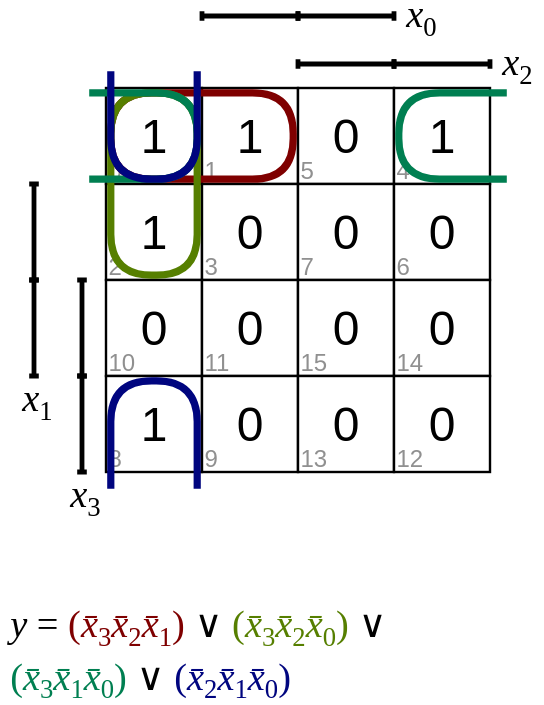
\includegraphics[width=.5\textwidth]{Exp03/2_2_karnaugh_map.png}
    \caption{Mapa de Karnaugh para o \textit{``Circuito de Minoria''}}\label{fig:2_2_karnaugh_map.png}
\end{figure}

Observando o mapa de Karnaugh, vemos que, por \textit{Soma de Produtos}, temos a
seguinte equação para \(Y_{2}\):

\begin{equation}
  Y_{2} = (\overline{A} \cdot \overline{B} \cdot \overline{C}) + (\overline{A} \cdot \overline{B} \cdot \overline{D}) + (\overline{A} \cdot \overline{C} \cdot \overline{D}) + (\overline{B} \cdot \overline{C} \cdot \overline{D})
\end{equation}

Entretanto, como devemos representar essa fórmula apenas em termos de portas
\textbf{NAND}, precisamos modificar a equação um pouco. Também temos a questão
de que esse circuito seria muito complexo para se implementar usando uma
conversão direta das \textbf{OR} para portas \textbf{NAND} requeridas no
enunciado. Por isso, também realizaremos alguns passos para minimização da
função booleana.

\begin{align}
  Y_{2} &= (\overline{A} \cdot \overline{B} \cdot \overline{C}) + (\overline{A} \cdot \overline{B} \cdot \overline{D}) + (\overline{A} \cdot \overline{C} \cdot \overline{D}) + (\overline{B} \cdot \overline{C} \cdot \overline{D})\\
  Y_{2} &= \overline{A}\cdot \overline{B} \cdot (\overline{C} + \overline{D}) + \overline{C} \cdot \overline{D} \cdot (\overline{A} + \overline{B})\\
  Y_{2} &= \overline{A}\cdot\overline{B} \cdot \overline{(CD)} + \overline{C}\cdot\overline{D} \cdot \overline{(AB)}\\
  Y_{2} &= \overline{\overline{ \left[ \overline{A}\cdot\overline{B} \cdot \overline{(CD)} \right] }} + \overline{\overline{ \left[ \overline{C}\cdot\overline{D} \cdot \overline{(AB)} \right] }}\\
  Y_{2} &= \overline{ \left( \overline{ \left[ \overline{A}\cdot\overline{B} \cdot \overline{(CD)} \right] } \cdot  \overline{ \left[ \overline{C}\cdot\overline{D} \cdot \overline{(AB)} \right] } \right)} \label{eq:2.2_NAND}
\end{align}

Possuindo a fórmula final \ref{eq:2.2_NAND} para o resultado \(Y_{2}\) desejado,
podemos criar um diagrama de mapeamento da função booleana para o circuito
lógico final:

\begin{figure}[H]
    \centering
    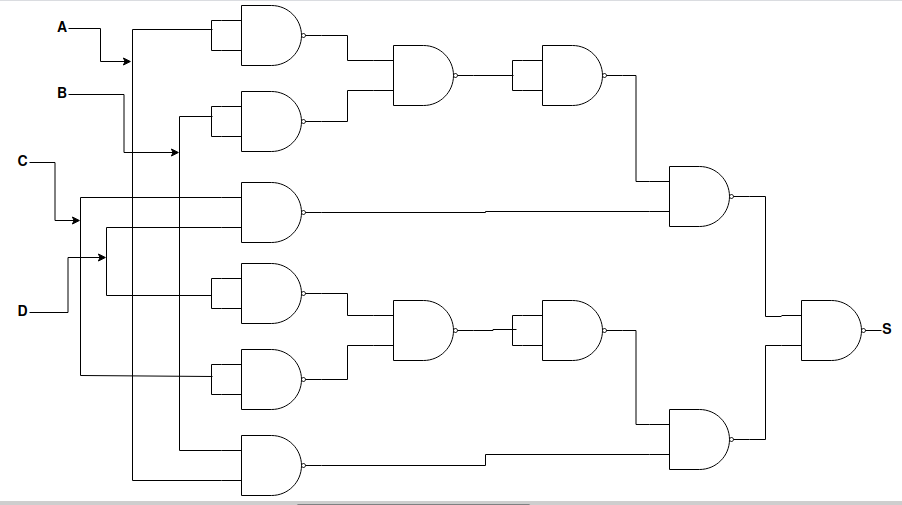
\includegraphics[width=.9\textwidth]{Exp03/2.2.png}
    \caption{Decisão de Minoria apenas com portas \textbf{NAND}}
    \label{fig:decisao_minoria}
\end{figure}

É possível concluir através da tabela, do diagrama, e da fórmula em
\ref{eq:2.2_NAND}, que de fato o circuito lógico final descreve uma decisão de
minoria com \(4\) entradas utilizando apenas usando portas \textbf{NAND}.

Como requisitado, apresentamos a montagem do circuito abaixo:

\begin{figure}[H]
    \centering
    \includegraphics[width=.9\textwidth]{Exp03/2.2_montagem.jpg}
    \caption{Montagem do circuito para \textit{Decisão de Minoria} apenas com portas \textbf{NAND}}
    \label{fig:decisao_minoria_montagem}
\end{figure}

Para conferir o vídeo deste experimento, acesse o seguinte link:
\href{https://youtu.be/7aZFW8PNZ44}{https://youtu.be/7aZFW8PNZ44}.
\\[2em]

\subsection{Circuito para \textit{``Decisão de Igualdade''} utilizando apenas portas \textbf{NAND}}\label{sec:decisao_igualdade}

O atual experimento visa implementar um circuito para \textit{Decisão de
Igualdade} utilizando somente portas \textbf{NAND}. O circuito deve ter 4 inputs
(\textbf{A}, \textbf{B}, \textbf{C} e \textbf{D}) e ter como output uma saída em
LED (\(Y_{3}\) \( = \) \textbf{L2}).

Esse experimento é muito semelhante aos anteriores, e fará uso dos circuitos
combinacionais já montados para produzir seu output.

Como desejamos fazer uma decisão de igualdade, e dado que já dispomos de um
circuito para decisão de maioria e outro para minoria, podemos lançar mão desses
circuitos para construir o desejado. Tal utilização dos já criados se dará da
seguinte forma: Sejam \textbf{S1} e \textbf{S2} as saídas lógicas dos circuitos
de maioria e minoria, respectivamente, temos que a saída do circuito de
igualdade, dado por \textbf{S3} deverá ser:

\begin{table}[H]
    \centering
    \caption{Decisão de Igualdade, baseado nos circuitos de Maioria e Minoria}
    \begin{tabular}{|c|c|c|}\hline
    \multicolumn{2}{|c|}{Entradas} & \multicolumn{1}{|c|}{Saída} \\\hline
    \textbf{S1} & \textbf{S2} & \textbf{S3} \\\hline
    0 & 0 & 1 \\\hline
    0 & 1 & 0 \\\hline
    1 & 0 & 0 \\\hline
    1 & 1 & * \\\hline
    \end{tabular}\label{tab:decisao_igualdade}
\end{table}

Cabe ressalvar que na tabela \ref{tab:decisao_igualdade}, a última linha possui
o valor de output ``\(*\)'' pois a entrada ``\(S1 = 1, \; S2 = 1\)'' é
logicamente impossível de ocorrer. Dessa forma, podemos atribuir o valor de
\emph{don't care} para esse output. Fazendo isso, passamos de uma função final
\(Y_{3} = S1 \cdot S2 + \overline{S1} \cdot \overline{S2}\) para uma forma mais
simplificada \(Y_{3} = \overline{S1} \cdot \overline{S2} \).

Por questão de completude, reproduziremos também a tabela verdade do circuito de
Decisão de Igualdade; Cabe ressaltar, entretanto, que não utilizamos mapa de
Karnaugh nem outro método para gerar essa tabela nem construir o circuito
lógico. O que fizemos, entretanto, foi utilizar as saídas dos circuitos de
Decisão de Maioria e Minoria.

\begin{table}[H]
    \centering
    \caption{Tabela Verdade para Decisão de Igualdade}
    \begin{tabular}{|c|c|c|c|c|}\hline
    \multicolumn{4}{|c|}{Entradas} & \multicolumn{1}{|c|}{Saída} \\\hline
    \textbf{D} & \textbf{C} & \textbf{B} & \textbf{A} & $\textbf{L2}=Y_{3}$ \\\hline
    0 & 0 & 0 & 0 & 0 \\\hline
    0 & 0 & 0 & 1 & 0 \\\hline
    0 & 0 & 1 & 0 & 0 \\\hline
    0 & 0 & 1 & 1 & 1 \\\hline
    0 & 1 & 0 & 0 & 0 \\\hline
    0 & 1 & 0 & 1 & 1 \\\hline
    0 & 1 & 1 & 0 & 1 \\\hline
    0 & 1 & 1 & 1 & 0 \\\hline
    1 & 0 & 0 & 0 & 0 \\\hline
    1 & 0 & 0 & 1 & 1 \\\hline
    1 & 0 & 1 & 0 & 1 \\\hline
    1 & 0 & 1 & 1 & 0 \\\hline
    1 & 1 & 0 & 0 & 1 \\\hline
    1 & 1 & 0 & 1 & 0 \\\hline
    1 & 1 & 1 & 0 & 0 \\\hline
    1 & 1 & 1 & 1 & 0 \\\hline
    \end{tabular}\label{tab:tabela_verdade_decisao_igualdade}
\end{table}

Como desejamos fazer uma decisão de igualdade, basta pegarmos o resultado da
\textit{Soma de Produtos} da tabela \ref{tab:decisao_igualdade} acima.

Dessa forma, concluímos que a saída \(Y_{3}\) desejada pode ser expressa da
seguinte forma:

\begin{equation}
  Y_{3} = S3 = \overline{S1} \cdot \overline{S2} \label{eq:2.3_NAND}
\end{equation}

Esquematicamente, teremos o seguinte diagrama:

\begin{figure}[H]
    \centering
    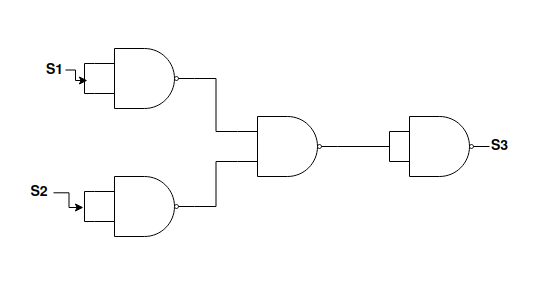
\includegraphics[width=.6\textwidth]{Exp03/2.3.png}
    \caption{Decisão de Igualdade, utilizando circuitos para Decisão de Maioria e Minoria}
    \label{fig:decisao_igualdade}
\end{figure}

É possível concluir através da tabela, do diagrama, e da fórmula em
\ref{eq:2.3_NAND}, que de fato o circuito lógico final descreve uma decisão de
minoria com \(4\) entradas utilizando apenas portas \textbf{NAND}.

Como requisitado, apresentamos a montagem do circuito abaixo:

\begin{figure}[H]
    \centering
    \includegraphics[width=.9\textwidth]{Exp03/2.3_montagem.jpg}
    \caption{Montagem do circuito para \textit{Decisão de Igualdade} apenas com portas \textbf{NAND}}
    \label{fig:decisao_igualdade_montagem}
\end{figure}

Para conferir o vídeo deste experimento, acesse o seguinte link:
\href{https://youtu.be/4czNGPVAp7s}{https://youtu.be/4czNGPVAp7s}.
\\[2em]

\section{Análise dos Resultados}
\label{sec:Resultados}

Através da utilização do teorema de Demorgan foi possível obter uma maior
minimização, sendo que indiretamente pode-se comprovar a veracidade do teorema,
e também pudemos aplicar a transição entre portas, ou seja, com portas \textbf{OR}
chegar a uma \textbf{AND}.

\section{Conclusão}
\label{sec:Conclusao}

Através dos experimentos realizados foi possível comprovar a universalidade de
portas \textbf{NAND}, pois pudemos, partindo de funções booleanas complexas
reduzí-las todas a funções que usassem apenas os operadores lógicos \emph{AND}
(\(\land\)) e \emph{NOT} (\(\lnot\)), mapeando posteriormente apenas para portas
\textbf{NAND}; Também pudemos ver, na prática, como o mapa de Karnaugh auxilia
na minimização de funções lógicas, reduzindo consideravelmente o número de
portas lógicas necessárias (claro, se pudessemos utilizar portas \textbf{NOR},
\textbf{OR}, etc nossos circuitos montados seriam menores).

\nocite{*}
\bibliographystyle{sbc}
\bibliography{relatorio}  %Aqui é a definição do arquivo .bib a ser usado pelas referências


\newpage
% Colocar aqui apenas as respostas dos itens da Auto-Avaliação
\section*{Auto-Avaliação}

Respostas:

\begin{table}[H]
    \begin{tabular}{|c|c|} \hline
    \textbf{A} & \textbf{B}\\
    \hline
    1 & b \\ \hline
    2 & d \\ \hline
    3 & c \\ \hline
    4 & a \\ \hline
    5 & d \\ \hline
    \end{tabular}
\end{table}


\end{document}
